%===========================================================
%                              Choix de track
%===========================================================
% Une des trois options 'parallelisme', 'architecture', 'systeme' 
% doit être utilisée avec le style compas2017
\documentclass[parallelisme]{compas2017}
\usepackage{rotating}
\usepackage{comment}
\usepackage{multirow}
\usepackage{graphicx}

\graphicspath{{gfx/}}

%===========================================================
%                               Title
%===========================================================

\toappear{1} % Conserver cette ligne pour la version finale

\begin{document}

\title{SCHIaaS : Un laboratoire d'études d'algorithmes par la simulation des clouds.}
\shorttitle{Simuler les clouds}

\author{Julien Gossa, Stéphane Genaud, Luke Bertot}% A voir l'ordre. 
% - Stéphane: moi en dernier.

\address{Université De Strasbourg,\\
Laboratoire ICube - Pôle API - 300 Bd Sébastien Brant\\
67400 Illkirch-Graffenstaden - France\\
julien.gossa@unistra.fr genaud@unistra.fr lbertot@unistra.fr}

\date{\today}

\maketitle

%===========================================================         %
%R\'esum\'e
%===========================================================  
\begin{abstract}

Les clouds ont été intensivement étudiés les dernières années, que ce soit du 
point de vue de l'administrateur qui doit par exemple décider de l'emplacement
des machines virtuelles sur l'infrastructure matérielle, ou du client qui doit 
décider du dimentionnement de sa plateforme virtuelle. Pour ce faire, de nombreux
simulateurs ont vu le jour. Malheureusement, ces derniers se limitent souvent à 
mimer les fonctionnalités d'un cloud. Ils ne proposent pas un cadre complet d'étude
des résultats obtenus, pourtant indispensable à la reproductibiltié des expériences
et la comparaison de solutions différentes. De plus, ils manquent d'ancrage dans la 
réalité, en raison d'une part d'une absence de comparaison à des exécutions réelles, 
et d'autre part d'un ensemble de traces réelles injectables dans les simulations.
Le projet SCHIaaS vise à combler ces deux manques. Nous montrons l'architecture de 
ce \textit{framework}, puis les résultats des expériences de validation.

  \MotsCles{un maximum de 5 mots significatifs, en français, doivent être 
    isolés sous forme de mots-clés.}
\end{abstract}


%=========================================================
\section{Introduction}
%=========================================================

Les  clouds  sont  devenus  ces  dernières  années  une  brique  essentielle  de
l'informatique,   omni-présents  dans   les   architectures   de  nos   systèmes
d'information. La compréhension de leurs  comportements est donc un enjeu majeur
qui a incité les chercheurs à proposer des simulateurs de cloud, essentiellement
pour les clouds de type \textit{Infrastructure-as-a-Service} (IaaS). Ces
simulateurs   reposent   sur   une   modélisation  qu'on   peut   qualifier   de
\textit{bottom-up} : les ressources matérielles sont d'abord modélisées, puis le
comportement des  machines virtuelles sur  ces ressources matérielles,  puis les
applications s'exécutant dans cet environnement. On peut donc distinguer dans 
de nombreux outils de simulation trois composants : 
\begin{itemize}
		\item une spécification de platforme
		\item une spécification de l'application.
		\item un modèle de simulation
\end{itemize}

Le modèle de simulation forme le coeur d'un simulateur. Il décrit l'évolution de
l'état de tous  les constituants du système  simulé en fonction du  temps et des
évènements.   Il  repose  sur  des   modèles  individuels  pour  chacun  de  ces
constituants  (réseau,  processeur,  \ldots).   Etant  donné  la  complexité  du
comportement   des   constituants,  les   modèles   actuels   procèdent  à   des
simplifications  générant  des  erreurs,   accentuées  par  la  combinaison  des
modèles. La précision des modèles utilisés est le principal élément discriminant
entre simulateurs, l'utilisateur  n'ayant généralement que peu de  prise sur cet
aspect%
\footnote{SimGrid  permet  néanmoins  de  choisir  différents  modèles  pour  le
  réseau}.

La spécification de plateforme décrit  l'environnement simulé.  Elle est fournie
par l'utilisateur et décrit les caractéristiques techniques de l'infrastructure,
comme la topologie  d'interconnexion, la puissance des  processeurs, la capacité
des liens réseaux,  etc.  Le niveau de détail de  cette description, qui différe
selon les simulateurs, influence la précision de la simulation.

La  spécification   de  l'application,   fournie  par  l'utilisateur,   est  une
description de la  séquence des évènements à simuler.  Les simulateurs existants
priviligient cette  description sous la forme  d'un programme qui, à  l'aide des
primitives  de  la  bibliothéque  de  simulation,  décrit  le  comportement  des
opération  réelles simulées.   Mais d'autres  mode de  description peuvent  être
proposés,   comme   l'injection  d'une   trace   d'exécution   réelle,  ou   une
représentation abstraite de suite d'opérations. La figure~\ref{fig:sim-features}
donne un aperçu des possibilités de différents simulateurs.


\begin{figure}[hbt]
\begin{tabular}{|c||c|c|c||c|c|c|c|}
	\hline
	%% line 1
	& \multicolumn{3}{c|}{Application} &
	\multicolumn{2}{c|}{CPU}&Réseau&Disque\\
	\cline{2-8}
	%%line 2
	Simulator &(a) 
                  &(b)
                  &(c)
                  &(d)
                  &(e)&
	type & precision max\\
	\hline
	%%line 3
	CloudSim\cite{cloudsim} & & & \bf X &&\bf
	X&store\&forward&seek+transfert\\ \hline
	ICanCloud\cite{icancloud} & & & \bf X &&\bf X&packet& bloc \\ \hline
	GroudSim\cite{groudsim} & & & \bf X &&\bf X&flot& n/a\\\hline
	GreenCloud\cite{greencloud} & & \bf X &&&\bf X&packet& n/a\\ \hline
	SimGrid\cite{simgrid}& \bf X & \bf X & \bf X &\bf X&\bf X& flot/packet &
	seek+transfert \\
	\hline
\end{tabular}
\caption{Principaux simulateurs du domaine et les possibilités de décrire
  l'application : (a) trace d'execution, (b) representation abstraite, (c) simulation
  programmée, ou la performance CPU : (d) delai mesuré, (e) délai
  utilisateur. Le réseau peut être simulé analytiquement (flow) ou avec un
  simulateur externe dédié (packet)}
\label{fig:sim-features}
\end{figure}

Cette description générale montre que la simulation d'une application exécutée
sur un cloud repose sur une combinaison de modèles qui par définition génèrent
une part d'erreur. La quantification de cette erreur est une tâche expérimentale
extrêmement fastidieuse, ce qui explique qu'elle est rarement menée. L'objet
de notre travail est ici de présenter un outil, le \emph{lab}, qui facilite
le travail d'analyse des résultats de simulation. Nous montrons comment cet 
outil peut être utilisé dans le cadre de la simulation d'application cloud
avec le \textit{framework} SCHIaaS qui repose sur SimGrid. Nous présentons 
d'abord cette interface dans la section~\ref{sec:schiaas}, puis blah blah.





%=========================================================
\section{Présentation du \textit{framework}}
%=========================================================

\subsection{SimGrid}

SimGrid~\cite{simgrid}  est un  simulateur à  évenements discrets  qui permet  à
l'utilisateur d'exprimer la modélisation  d'une application distribuée à travers
un  programme utilisant  les  primitives  SimGrid qui  décrivent  les phases  de
communications et de calcul des différents processus applicatifs. Ces primitives
sont disponibles à travers différentes interfaces, adaptées aux systèmes étudiés
; il  existe par exemple  des interface  pour les applications  pair-à-pair, MPI
(SMPI),  les workflows  sous forme  de DAG  (SimDAG), \ldots,  ou les  processus
communiquants de type  CSP (MSG). Dans cet article nous  présentons une nouvelle
interface, SCHIaaS,  dédiée à la simulation  de clouds IaaS. Celle-ci  est basée
sur l'interface MSG.



SCHIaaS est un \textit{framework} permettant le développement rapide de simulateurs 
de cloud pour l'évaluation d'algorithmes au niveau du \textit{cloud-kit} et au dessus.
Il est basé sur SimGrid et est développé en JAVA, ce qui permet la spécialisation 
rapide d'un ensemble de classes permettant de greffer les travaux de l'utilisateur au 
niveau qui lui convient, le reste étant assuré par défaut.
Le tout est facilement instrumentable par un ensemble de scripts, appelé \emph{lab},
qui permet d'automatiser l'exécution des simulations, leurs observations, et l'analyse
des résultats.

Schema :

lab (lab.py + schiaas-trace-utils.py )

applications (simschlouder, loadinjector, \ldots)

schiaas (engines + apps)

simgrid (vm + msg)


\subsection{SCHIaaS}

SCHIaaS est la sur-couche de SimGrid, qui ajoute par dessus l'interface MSG toutes les 
fonctionnalités d'un cloud. 
Le niveau \textit{cloud-kit} est assuré par mes moteurs, exposant les fonctionnalités 
des clouds au niveau administrateur :
\begin{itemize}
 \item Compute : moteur d'instanciation et de gestion des VM;
 \item Storage : moteur de gestion des stockages;
 \item Network : moteur de gestion de la virtualisation du réseau (à l'état purement abstrait pour l'instant).
\end{itemize}

Chacun de ces moteurs est une interface abstraite, qui assure l'interopérabilité entre eux, 
ainsi qu'avec les autres niveaux du \textit{framework}. Des implémentations sont fournies, qui 
permettent d'obtenir un simulateur par défaut pleinement fonctionnel. Ces implémentations 
imitent le comportement d'openstack. Un développeur de fonctionnalités administrateur n'a donc 
qu'à se concentrer sur la partie qui l'intéresse, par exemple différent systèmes de stockages.

Les ordonnanceurs de VM, qui décident sur quelle PM seront déployées les VM demandées
par l'utilisateur, ont également leur interface abstraite. Plusieurs ordonnanceurs par défaut
sont fournis, sur l'exemple d'Openstack qui permet au choix d'équilibrer ou de consolider les 
charges des machines physiques au moyen d'un poids calculé pour chacune d'elles. 

Un système abstrait d'injection de charge est également fourni. Ce dernier permet de contrôler 
un nombre de VM déployées et les charges de ces VM, en particulier CPU, afin de faciliter 
l'évaluation des algorithmes.
Deux injecteurs par défaut sont fournis. Le premier est un simple injecteur de charges sinusoidales
entièrement paramétrables. Le second injecte les charges observées sur l'infrastructure de Google,
et rendue disponible dans le google-cluster-traces.

Ces interfaces ne sont que celles utilisées dans la suite de l'article à titre d'illustration.
De la même manière, SCHIaaS fourni de façon modulaire tous les composant d'un \textit{cloud-kit}. 
Chaque module peut être remplacé, étendu, ou utilisé en l'état, ce qui permet le prototypage
rapide de simulateurs de cloud adaptés à l'étude de l'utilisateur, sans qu'il ait à développer 
plus que ce qui l'intéresse.

\subsection{Applications}

SCHIaaS ne peut s'exécuter seul. Dans la philosophie SimGrid, un simulateur est une application
exploitant les fonctionnalités fournies, mais qui doit être développée et compilée.
Cette philosophie est conservée avec SCHIaaS, qui ne fait qu'étendre les fonctionnalités de 
SimGrid avec celles disponibles dans un cloud.

Cependant, deux applications sont fournies par défaut: 
\begin{itemize}
 \item \emph{LoadInjector}, qui permet d'injecter une charge utilisateur sans se préoccuper
 des applications qui s'exécutent dans les VM. Il est utile pour mener des études au niveau 
 administrateur.
 \item \emph{SimSchlouder}, qui est la version simulée du système réel Schlouder\cite{Michon2017}.
 Il s'agit d'un courtier de ressources virtuelles capable de piloter de concert un ordonnanceur de tâches 
 et un \textit{cloud-kit} pour exécuter des calculs scientifiques sur clouds. 
 Schlouder et SimSchlouder ont exactement les mêmes entrées/sorties, excepté le résulat 
 des calculs effectués, ce qui permet de mener des études au niveau utilisateur de cloud,
 sans se préoccuper du niveau administrateur. De plus, ceci permet de confronter les 
 performances simulées aux performances réelles, et donc de valider la précision de 
 la simulation. Cela a été fait sur la base de 273 exécution réelles, incluant 8 cas applicatifs
 représentatifs et 4 plateformes de cloud représentatives. Cette validation est en cours 
 de publication. Les traces d'exécution réelles sont inclues dans SimSchlouder afin de 
 pouvoir servir à la validation des travaux sur le calcul scientifique sur cloud.
\end{itemize}

\subsection{Le Lab}

Le lab est un ensemble de scripts permettant d'automatiser l'exécution des simulations, la collecte des
observations, ainsi que leur analyse. Il permet donc d'exécuter de bout-en-bout l'étude par simulation,
de la définition des différentes simulations, à la production des graphiques.

Au delà de l'aspect pratique et du gain de temps de mise en oeuvre de l'étude, le lab a pour vocation
de ``standardiser'' l'étude. Cette standardisation assure sa reproductibilité, ainsi qu'une comparaison
équitable entre solutions à un même problème.

Mais le lab permet également une approche systématique permetant à l'expérimentateur de ne pas rater 
de phénomène. En effet, il est fréquent de faire un grand lot de simulations, plus d'observer plus
finement celles qui présentent des particularités. Ce faisant, l'expérimentateur exclu les autres 
simulation de ces observations plus précises, à moins de les refaire entièrement. En rendant plus 
pratique la définition des observations directement au niveau du \textit{workflow} de simulations, 
le lab assure que tous les cas seront observés de la même manière, ce qui évite de rater un phénomène,
ou de différencier le traitement des simulations au risque d'arriver à des conclusions abusives.


\section{Cas d'usage concret}

Afin d'illustrer 

L'application \emph{LoadInjector} permet le prototypage rapide de simulateurs
pour évaluer les algorithmes du niveau \textit{cloud-kit}. Dans ces cas là,
seule compte la charge en terme de nombre de VMs et de CPU de ces VMs, peu
importe les applications qui y sont exécutées.

Le conception d'un systeme systeme d'ordonnancement ce fait par l'extention de
la classe \emph{ComputeScheduler}. N'importe quel classe satifessant l'interface
peut etre chargé a l'initialisation de SCHIaaS ce qui permet de prototypé
facilement de nouveaus ordonnanceurs. De base SCHIaaS fournit : 
\begin{description}
	\item[SimpleScheduler], un ordonanceur pondéré pouvant être configuré de
		manière a répartir (\emph{balancer}) ou concentré
		(\emph{consolidator}) les VMs sur les PMs
	\item[SimpleReconfigurator], ce base sur \emph{SimpleScheduler} tente
		régulièrement d'optimiser le placement des VMs en procédant à
		des migration.
\end{description}

Pour mettre nos ordonnanceurs à l'épreuve notre ordonnanceur il va être
nécessaire de provisionner des VMs dans notre simulation. Comme la charge
applicative ne fait pas partie du cadre de cette expérience on utilisera
\emph{LoadInjector}. La classe \emph{loadinjector.SimpleInjection} permet de
lancer des simulation autour d'injecteurs implémentant la classe
\emph{AsbstractInjector}. Les injecteurs allume des VMs, leur assigne des
charges de calcul et les éteignes. SCHIaaS fournit \textbf{SinInjector} qui
injecte une charge de calcul sinusoïdale sur un nombre de VM suivant aussi une
sinusoïde. L'exécution d'une simulation ce fait avec la commande suivante : 
\begin{verbatim}
$ java  loadinjector.SimpleInjection platform.xml deploy.xml cloud.xml
injector.xml
\end{verbatim}
\begin{description}
	\item[platform.xml] décrit les PMs pour SimGrid
	\item[deploy.xml] instancie les processus SimGrid
	\item[cloud.xml] décrit le cloud, en particulier l'ordonnanceur a
		utiliser pour SCHIaaS
	\item[injector.xml] sélectionne et paramètre les injecteurs a utiliser
\end{description}

\subsubsection{Cas d'usage}

Dans ce cas d'usage on imagine que l'on cherche a optimiser la configuration d'un
ordonnanceur cherchant a limiter le nombre de PM utilisé. Pour ce faire on va
comparer la performance des ordonnanceur suivant : 
\begin{description}
	\item[SimpleScheduler : balancer] : cas témoin
	\item[SimpleScheduler : consolidator] : cas témoin
	\item[SimpleReconsolidator : 10] : cherche a optimisé l'ordonnancement
		en migrant une VM toute les 10 secondes.
	\item[SimpleReconsolidator : 100] : cherche a optimisé l'ordonnancement
		en migrant une VM toutes les 100 secondes
\end{description}

Pour couvrir un maximum de cas possible on modèle 3 profils d'injection, un
variant lentement, un variant rapidement, et commençant lentement avant de
varier rapidement.

Tous les ordonnanceurs et tous les injecteur sont décrit dans des fichier
\emph{cloud} et \emph{injection} respectivement. Il existe 15 combinaison
ordonnanceur/injecteur à simuler et à comparer. Le \emph{lab} va entièrement
automatisé les étapes de simulation et d'analyse.

\subsubsection{Configuration du lab}

Toutes les expérience du \emph{lab} sont guidée par un fichier de configuration.
Celui ci contient l'ensemble des information nécessaire aux simulations, les
variables à observer, et si nécessaire les pré- ou post- traitement requis. 

\begin{verbatim}
# setup
SETUP_DIR ./setup/cmp-scheduler
NEEDED_POST template.R
POST_COMMAND_DATA R -f template.R > R.out

# observations
TU_ARG --grep vm:.*:state
TU_ARG --event instances_count 
TU_ARG --event used_cores
TU_ARG --event instances_load 
TU_ARG --event cpu_bound
TU_ARG --count-if used_cores ne 0
TU_ARG --count-if used_cores eq 0
TU_ARG --count-if vm:.*:state eq migrating
TU_ARG --count-if vm:.*:state eq running

# simulations
SIM_ARG 1 loadinjector.SimpleInjection
SIM_ARG 2 platform.xml 
SIM_ARG 3 deploy.xml
SIM_ARG 4:balancer cloud-balancer.xml
SIM_ARG 4:consolidator cloud-consolidator.xml
SIM_ARG 4:reconsolidator10 cloud-reconsolidator10.xml 
SIM_ARG 4:reconsolidator100 cloud-reconsolidator100.xml
SIM_ARG 5:slow injector-slow.xml
SIM_ARG 5:fast injector-fast.xml
SIM_ARG 5:slowfast injector-slowfast.xml 
\end{verbatim}

\begin{enumerate}
	\item Mise en place
		\begin{description}
			\item[SETUP\_DIR] dossier où se trouve tout les fichiers
			\item[POST\_COMMAND\_DATA] commande a exécuter sur les
				observations
			\item[NEEDED\_POST] fichiers requit par POST\_COMMAND\_DATA 
		\end{description}
		Il est possible d'exécuter des commandes avant simulation
		(PRE\_COMMAND\_SETUP), ou d'injecter d'autre fichier de commande
		(INCLUDE) eventuelement eux même écrit par la précommande.
	\item Simulations
		\begin{description}
			\item[SIM\_ARG $n$:nom] ensemble des argument a
				passer au simulateur indexé par leur position
				$n$. Le \emph{lab} entreprendra une simulation
				pour chaque combinaison d'argument possible.
				Pour que index ou plusieurs argument sont
				possible un nom et requit pour différencié les
				simulations.
		\end{description}
		Les l'ensemble des fichiers écrit par chaque simulation sont placé
		dans un dossier nommé d'après les argument de la simulation.
	\item Observation
		\begin{description}
			\item[TU\_ARG] ensemble de filtre a appliquer au traces
				de simulation.
		\end{description}
		Les fichier obtenu grâce a TU\_ARGS permettent d'observer les
		variables pertinente de la simulation sans avoir a fouiller
		l'ensemble des traces verbeuses de SCHIaaS. Cette étape est
		cruciale pour l'exploitation automatique des résultats
\end{enumerate}

La commande \texttt{./lab.py -p 4 [-k] cmp-scheduler.cfg} permet d'exécuter cet
expérience. L'option \texttt{p} indique le nombre de simulation a mené en
parallèle et l'option \texttt{k} permet de sauter la simulation pour faire les
observations sur les trace d'un simulation précédente.

\subsubsection{Analyse des résultats}

Le \emph{lab} a exécuté toute les simulation et extrait les informations utiles
de chacune des trace.Ces observation sont disponible dans le dossier
\texttt{data} en tant que fichiers de la forme:
\begin{verbatim}
xp[_nom1[_nom2[...]]].observ.dat
\end{verbatim}
Avec \texttt{nom$n$} sont les noms donnés au SIM\_ARG utilisé pour cette
simulation et \texttt{observ} le filtre TU\_ARG utiliser pour obtenir ce
fichier. Le \emph{lab} n'integre pas plus de traitement pour ces données, mais
permet au utilisateur de lancer de manière systématique une commande
supplémentaire dans le fichier \texttt{data}. Dans notre cas il s'agit d'un
script R utilisant une bibliothèque fournie avec le \emph{lab} pour tracer les
variables observé dans un graphe approprié et d'écrire tout les graphe dans PDF.

\begin{figure}[h]
	\label{output}
	\caption{Exemple de graphe obtenu par le TU\_ARGS :
	\texttt{instances\_count}(event), \texttt{vm:.*:state eq running}(count-if)
	et, \texttt{vm:.*:state}(grep)}
	\begin{tabular}{ccc}
		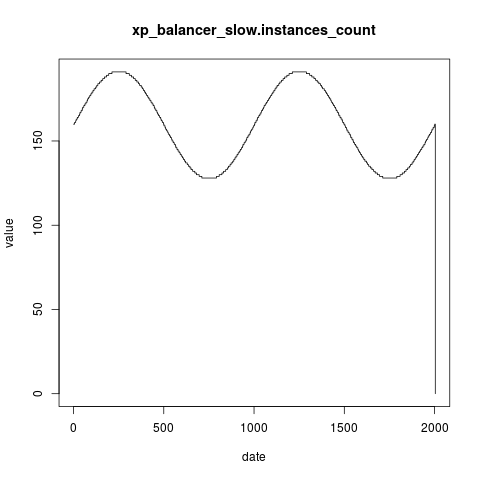
\includegraphics[scale=0.30]{xp_balancer_slow-instances_count}&
		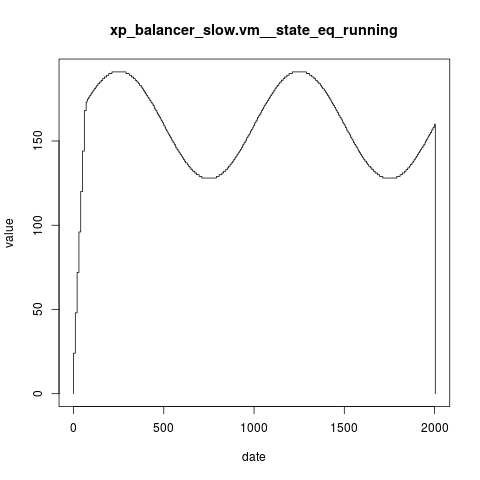
\includegraphics[scale=0.30]{xp_balancer_slow-vm__state_eq_running}&
		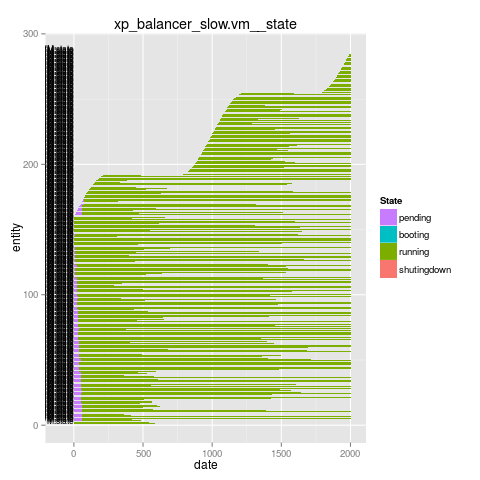
\includegraphics[scale=0.30]{xp_balancer_slow-vm__state}\\
	\end{tabular}
\end{figure}

\section{Conclusion}

Le \emph{lab} est un outil pour l'automatisation d'exécution d'expériences
\emph{in silico} qui permet chainé facilement de multiple simulation en faisant
varié les entrées. L'automatisation des simulation et des observation permet non
seulement de s'assurer que rien n'échappe a l'utilisateur mais rend aussi
l'expérience trivialement reproductible. Le \emph{lab} est déjà utilisé au seins
de notre équipes pour la validation de SCHIaaS, en simulant automatiquement
l'ensemble d'une archive de 273 exécution réelle, et pour des simulation de
Monte Carlo, en procédant de manière répétée a 500 simulations d'une même
plateforme avec des taches généré aléatoirement. ???






%=========================================================
\section{Exemples}
%=========================================================

\subsection{Comparaison d'algorithmes de placement de VM sur PM}

\subsection{Comparaison d'algorithmes d'ordonnancement de tâches sur VM}

\section{Open-science}

\begin{verbatim}
git clone https://git.unistra.fr/gossa/schlouder-traces.git
git clone https://scm.gforge.inria.fr/anonscm/git/schiaas/schiaas.git 
cd schiaas
cmake .
make
cd lab
./lap.py -p2 setup/simschlouder/validation.cfg
cd setup/simschlouder/validation-results
ls
\end{verbatim}


\bibliography{biblio}

\end{document}



\subsection{SimSchlouder}

L'application \emph{SimSchlouder} permet le prototypage rapide de simulateurs pour évaluer les 
algorithmes d'ordonnancement de VM et de tâches au niveau utilisateurs du cloud. 
Dans ces cas là, l'état de l'infrastructure interne du cloud importe peu, seule compte le service 
rendu à l'utilisateur, isolé sur sa propre plateforme virtuelle. 

Schlouder\cite{Michon2017} est un courtier de ressources virtuelles. Il prend en
entrée la description d'une charge de travail, au format slurm citation???
étendu de quelques informations permettant d'adapter le courtage aux besoins
utilisateurs. Ensuite, Schlouder anaylse la charge de travail soumise, et décide
à l'aide d'algorithmes de dimensionnement (\textit{provisioning}) de déployer un
certains nombres de VM, puis ordonnance les tâches sur ces VMs, et étend les VMs
lorsqu'elles sont devenues inutiles.

SimSchlouder est l'alter-égo de Schlouder, dont l'architecture, les fonctionnalités, le comportement
et les entrées/sorties sont entièrement reproduite dans SCHIaaS. La description d'une charge de 
travail peut donc être soumise indifférement à Schlouder pour une exécution réelle, ou à SimSchlouder
pour une évaluation des choix de courtage par la simulation. Une option de Schlouder permet 
d'ailleurs d'appeler directement SimSchlouder, et d'obtenir le temps de completion et le prix 
de l'exécution demandée en fonction de la plateforme de cloud cible et de la stratégie de réservation
de VM choisie.

Les stratégies d'évaluation des réservations de ressources de cloud ont été intensivement étudiées 
ces dernières années. Cependant, elles sont rarement comparées entre elles, et leur évaluation 
est souvent basée sur des simulations ad-hoc ou inadaptées, et des charges de travail purement artificielles.
SimSchlouder permet de rapidement développer de telles stratégies, et de comparer leurs performances 
à celles fournies par défaut, à savoir ASAP (\textit{As Soon As Possible}, qui vise à minimiser le temps de 
complétion) et AFAP (\textit{As Full As Possible}, qui vise à minimiser les réservations de ressources,
et donc le coût). De plus, cette comparaison peut s'appuyer sur les traces récupérées lors de l'utilisation 
de l'application réelle Schlouder. Pour l'instant, nous mettons à disposition 481 traces d'exécutions
sur deux plateformes : notre cloud privé, homogène, stable et non partagé, et BonFire qui est un cloud 
public hétérogène, instable et partagé, dont les différents sites ont des comportements et des matériels 
assez différents pour qu'on les considère ocmme des clouds différents.
Les charges de travail sont issues de deux applications : OMSSA, qui est un sac de tâches assez courtes 
en protéomique, et MONTAGE, qui est un \textit{workflow} en astronomie ayant des tâches plus imposantes. 

Ainsi, l'utilisation de SimSchlouder permet de ne développer que le coeur d'un stratégie de résevation 
de resources, simplement en implémentant une interface abstraite très simple, pour pouvoir comparer cette 
stratégie aux autres dans des contextes applicatifs et matériels nombreux, représentatifs, et réellement 
éprouvés.

Ces comparaisons nécessitent de très nombreuses simulations, c'est pourquoi nous avons conçu \emph{le lab}.
